\section{202109-3 脉冲神经网络}
	\begin{itemize}
		\item 时间限制:$1.0\texttt{ s}$.
		\item 空间限制:$512.0\texttt{ MiB}$.
	\end{itemize}
	\subsection{题目}
		\subsubsection{题目背景}
			在本题中,你需要实现一个 SNN(spiking neural network,脉冲神经网络)的模拟器。一个 SNN 由以下几部分组成:
			\begin{enumerate}
				\item 神经元:按照一定的公式更新内部状态,接受脉冲并可以发放脉冲
				\item 脉冲源:在特定的时间发放脉冲
				\item 突触:连接神经元-神经元或者脉冲源-神经元,负责传递脉冲
			\end{enumerate}
		\subsubsection{题目描述}
			\par 神经元会按照一定的规则更新自己的内部状态。本题中,我们对时间进行离散化处理,即设置一个时间间隔 $\Delta t$,仅考虑时间间隔整数倍的时刻 $t=k\Delta t(k\in\mathbb{Z}_+)$,按照下面的公式,从 $k-1$ 时刻的取值计算 $k$ 时刻变量的取值:
			$$v_k=v_{k-1}+\Delta t(0.04v_{k-1}^2+5v_{k-1}+140-u_{k-1})+I_k$$
			$$u_k=u_{k-1}+\Delta ta(bv_{k-1}-u_{k-1})$$
			其中 $v$ 和 $u$ 是神经元内部的变量,会随着时间而变化,$a$ 和 $b$ 是常量,不会随着时间变化;其中 $I_k$ 表示该神经元在 $k$ 时刻接受到的所有脉冲输入的强度之和,如果没有接受到脉冲,那么 $I_k=0$。当进行上面的计算后,如果满足 $v_k\geq 30$,神经元会发放一个脉冲,脉冲经过突触传播到其他神经元;同时,$v_k$ 设为 $c$ 并且 $u_k$ 设为 $u_k+d$,其中 $c$ 和 $d$ 也是常量。图 1 展示了一个神经元 $v$ 变量随时间变化的曲线。
			
			\par 突触表示的是神经元-神经元、脉冲源-神经元的连接关系,包含一个入结点和一个出结点(可能出现自环和重边)。当突触的入结点(神经元或者脉冲源)在 $k$ 时刻发放一个脉冲,那么在传播延迟 $D(D>0)$ 个时刻以后,也就是在 $k+D$ 时刻突触的出结点(神经元)会接受到一个强度为 $w$ 的脉冲。
			\par 脉冲源在每个时刻以一定的概率发放一个脉冲,为了模拟这个过程,每个脉冲源有一个参数 $r$ ,并统一采用以下的伪随机函数:
			\par C++ 版本:
			\lstinputlisting[
				style=C++
			]{problem3.cpp}
			\par 在每个时间刻,按照编号顺序从小到大,每个脉冲源调用一次上述的伪随机函数,当 $r>\operatorname{myrand}()$ 时,在当前时间刻发放一次脉冲,并通过突触传播到神经元。
			\par 进行仿真的时候,已知 $0$ 时间刻各个神经元的状态,从 $1$ 时间刻开始按照上述规则进行计算,直到完成 $T$ 时刻的计算,再输出 $T$ 时刻神经元的 $v$ 值和发放的脉冲次数分别的最小值和最大值。
			\par 规定输入数据中结点按如下方式顺序编号:$[0,N-1]$ 为神经元的编号,$[N,N+P-1]$ 为脉冲源的编号。
			\par 代码中请使用双精度浮点类型。
		\subsubsection{子任务}
			\begin{table}[!ht]
				\centering
				\begin{tabular}{|c|c|c|c|c|c|c|}
				\hline
					子任务 & $T$ & $N$ & $S$ & $P$ & $D$ & 分值 \\ \hline
					1 & $10^2$ & $10^2$ & $10^2$ & $10^2$ & $10^2$ & $30$ \\ \hline
					2 & $10^3$ & $10^3$ & $10^3$ & $10^3$ & $10^3$ & $40$ \\ \hline
					3 & $10^5$ & $10^3$ & $10^3$ & $10^3$ & $10$ & $30$ \\ \hline
				\end{tabular}
			\end{table}
	\subsection{解法 A(30 分)}
		\subsubsection{原理阐释}
			\par 按秒维护,每秒处理神经元时枚举邻接情况,用邻接矩阵处理,则处理单个神经元复杂度为 $\Theta((n+p)D)$。
			\par 从而总的时间复杂度为 $\Theta(Tn(n+p)D)$,空间复杂度为 $\Theta((n+p)^2)$。
	\subsection{解法 B(70 分)}
		\subsubsection{原理阐释}
			\par 与解法 A 相同的思路,但换用邻接表存图,此时每一秒处理每个神经元产生脉冲的总的复杂度就变为 $\Theta(sD)$。
			\par 从而总的时间复杂度为 $\Theta(T(n+sD+p))$,空间复杂度为 $\Theta(n+p+s)$。
			\par 实际上本解法因为题目时间限制过于紧张,只能拿到 $66$ 分。
	\subsection{解法 C(100 分)}
		\subsubsection{原理阐释}
			\par 若每次都枚举 $D$ 时刻之前各个神经元的状态,则代价十分昂贵。注意到 $D$ 很小,则我们可以用滚动数组直接存储其余神经元对特定神经元在特定时间贡献的总和。
			\par 这个值每次处理神经元产生脉冲时直接简单相加,处理神经元新状态时读取并清空即可。
			\par 总的时间复杂度为 $\Theta(T(n+p+s))$,空间复杂度为 $\Theta(nD+n+p+s)$。
			\par \textbf{由于时间限制过于紧张,如果仅仅按照上面的思路编写代码难以通过,下面我将介绍几种在不使用其他条件的情况下加速程序的办法。}
			\begin{enumerate}
				\item \textbf{取模优化}:若对于两个都在完全剩余类中的数,它们的加法取模可以转化为简单的加法和减法,见代码中的 ``add'' 函数;
				\item \textbf{局部性优化}:增强代码的局部性,对于神经元的三个步骤(更新,清空滚动数组,脉冲)分开处理,增强代码的内存局部性从而利用 CPU 缓存加速。
				\item \textbf{预处理优化}:简化题目给定的表达式,将冗余的计算参数提前算好,见代码中的 ``A,B,C'' 参数和 ``ap''。
				\item \textbf{浮点优化}:题目虽然要求使用 ``double'' 类型的浮点数,但可以发现,题目的算数有效位数很低,可以在某些精度要求不高的变量(除了 $u, v, \Delta t$ 都要求不高)上使用 ``float'' 类型,加速浮点运算。
				\item \textbf{循环展开}:这题的计算稍有复杂之处,若欲有效循环展开则需要使用额外空间存储中间变量,内存限制稍紧,故不采用。
			\end{enumerate}
		\subsubsection{C++ 代码实现}
			这份代码使用了取模优化、局部性优化、预处理优化、浮点优化,其中取模优化更进一步,利用了位运算优化。可以轻松通过本题。
			\lstinputlisting[
				style=C++,
				title={\bf 202109-3.cpp},
				tabsize=4
			]{202109-3.cpp}
		\subsubsection{提交结果}
			\begin{figure*}[htbp]
				\centering
				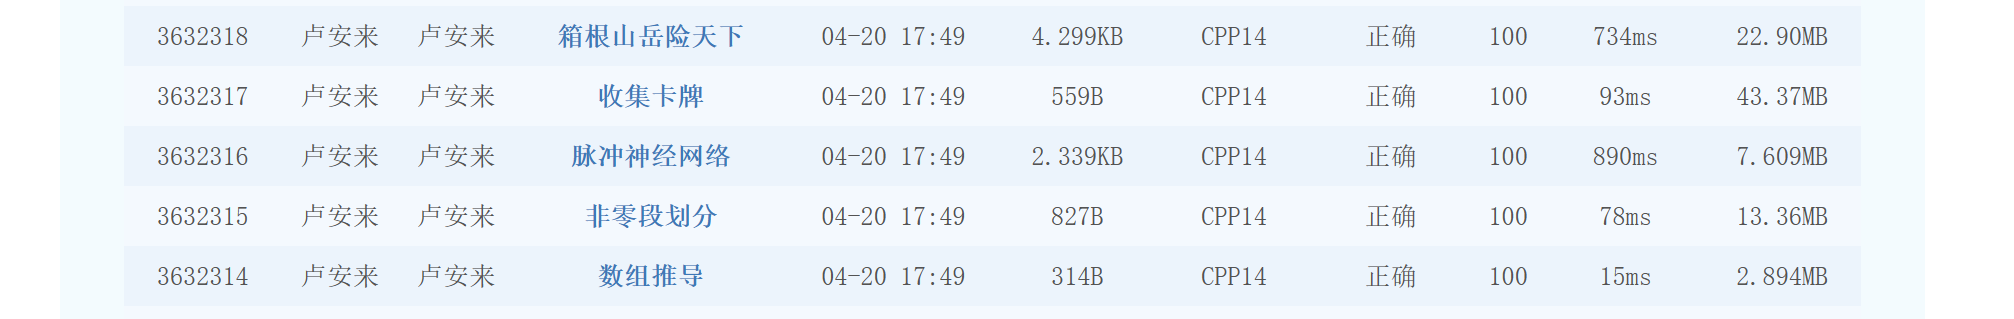
\includegraphics[width=1\textwidth]{result.png}
				\caption{提交结果}
			\end{figure*}